% =====================================================================
%  Sustentación del trabajo de grado · tema SHZU (shzu.sty)
%  Compilar:  latexmk -pdf main.tex   (pdfLaTeX; en Overleaf, pdfLaTeX)
%  Contenido por sección en secciones/*.tex
%  Complementos (cajas, colores, diagramas) en uisextras.sty
% =====================================================================
\documentclass[aspectratio=169]{beamer}

\usepackage[utf8]{inputenc}
\usepackage[T1]{fontenc}
\usepackage{lmodern}
\usepackage[spanish,es-noshorthands,es-nodecimaldot]{babel}
\usepackage{amsmath,amssymb}
\usepackage{booktabs,tabularx,array}
\usepackage{pgfplots}
\pgfplotsset{compat=1.18}
\usepackage{appendixnumberbeamer}
\usepackage{fontawesome5}

\title[Agente DVFS con modelos ligeros de ML]{Diseño e Implementación de un Agente en
Espacio de Usuario para la Gestión Dinámica de Frecuencia (DVFS) en Sistemas
Heterogéneos mediante Modelos Ligeros de Machine Learning}
\subtitle{Trabajo de grado · Modalidad Investigación}
\author[Cáceres Torres · Pérez Porras]{Yeison Adrián Cáceres Torres \and Ricardo Andrés Pérez Porras\\[1mm]
  {\footnotesize Director: Gilberto Javier Díaz Toro, Ph.D.}}
\institute[UIS · Escuela de Ingeniería de Sistemas e Informática]{Universidad Industrial de Santander\\
  Escuela de Ingeniería de Sistemas e Informática}
\date{}  % fecha de la sustentación

\usepackage{shzu}
\usepackage{uisextras}
% El tema repite la tabla de contenido al inicio de cada sección; aquí sin
% subsecciones para que quepa. Para quitarla: \AtBeginSection[]{}
\AtBeginSection[]{
  \begin{frame}
    \begin{columns}[T]
      \begin{column}{0.48\textwidth}
        \tableofcontents[sections={1-4},currentsection,hideallsubsections]
      \end{column}
      \begin{column}{0.48\textwidth}
        \tableofcontents[sections={5-8},currentsection,hideallsubsections]
      \end{column}
    \end{columns}
  \end{frame}
}
\graphicspath{{figuras/}}

\begin{document}

\begin{frame}
  \titlepage
  \vspace{-5mm}
  \begin{center}
    
\includegraphics[height=7mm]{logos/cage.png}\hspace{4mm}%
    
\includegraphics[height=7mm]{logos/uis.png}
  \end{center}
\end{frame}

\begin{frame}{Contenido}
  \begin{columns}[T]
    \begin{column}{0.48\textwidth}
      \tableofcontents[sections={1-4},hideallsubsections]
    \end{column}
    \begin{column}{0.48\textwidth}
      \tableofcontents[sections={5-8},hideallsubsections]
    \end{column}
  \end{columns}
\end{frame}

% ---------------------------------------------------------------------
%  01 · Contexto
%  Ideas de la presentación original (nodo heterogéneo, potencia y energía,
%  costo y disponibilidad, DVFS depende de la fase). Un ícono grande y una
%  frase corta por columna; el resto, de viva voz.
% ---------------------------------------------------------------------
\seccion{Contexto}

% \ctxcol{ícono}{título}{frase}  (columna de ancho fijo, tarjeta con ícono grande)
\newcommand{\ctxcol}[3]{%
  \begin{minipage}[t]{0.3\textwidth}
    \centering
    \tikz[baseline=0]\node[circle,fill=uisgreen,text=white,minimum size=17mm,inner sep=0pt,
      font=\fontsize{20}{22}\selectfont]{#1};\par\vspace{3mm}
    {\large\bfseries\color{uisgreen}#2\par}\vspace{1.5mm}
    {\small #3\par}
  \end{minipage}}

\begin{frame}{La energía limita cuánto puede escalar un nodo CPU--GPU}
  \vspace{4mm}
  \centering
  \ctxcol{\faMicrochip}{Nodo heterogéneo}{CPU y GPU comparten la carga científica}\hfill
  \ctxcol{\faBolt}{Potencia y energía}{Cada dispositivo consume según su frecuencia y su actividad}\hfill
  \ctxcol{\faLeaf}{Costo y disponibilidad}{La energía incide en los costos operativos y en la sostenibilidad}

  \vspace{7mm}
  \begin{cardhi}[halign=center,fontupper=\normalsize,top=3mm,bottom=3mm,width=0.88\textwidth,center]
    DVFS ajusta voltaje y frecuencia en el hardware, pero\\
    \textbf{el beneficio depende de lo que hace la aplicación en cada fase}
  \end{cardhi}
\end{frame}

% ---------------------------------------------------------------------
%  02 · Problema
% ---------------------------------------------------------------------
\seccion{Problema}

\definecolor{uismem}{HTML}{8DBF2E}   % lima oscuro: legible sobre blanco

% Tarjeta de una fase: cabecera con el color de la fase, gráfico T(f) y resultado.
% \phasecard{color de relleno}{color del texto de la cabecera}{título}{curva}{resultado}
\newcommand{\phasecard}[5]{%
  \begin{minipage}[t]{0.47\textwidth}
    \begin{tcolorbox}[uisbase,colback=uiscard,height=50mm,valign=center,halign=center,
      left=3mm,right=3mm,top=2mm,bottom=2mm]
      \tikz[baseline=-0.6ex]\node[rounded corners=0.8mm,fill=#1,text=#2,font=\small\bfseries,
        minimum width=34mm,minimum height=6mm]{#3};\par\vspace{2mm}
      \begin{tikzpicture}[x=0.5mm,y=0.3mm]
        \draw[uisgray2,line width=0.8pt,-{Latex[length=1.6mm]}] (0,0) -- (0,52);
        \draw[uisgray2,line width=0.8pt,-{Latex[length=1.6mm]}] (0,0) -- (96,0);
        \node[font=\scriptsize\bfseries,anchor=east] at (-2,50) {$T$};
        \node[font=\scriptsize\bfseries,anchor=north] at (94,-3) {$f$};
        \draw[#1,line width=2.4pt,domain=0:90,samples=40,smooth] plot (\x,{#4});
      \end{tikzpicture}\par\vspace{1mm}
      {\normalsize\bfseries #5\par}
    \end{tcolorbox}
  \end{minipage}}

\begin{frame}{Una misma aplicación alterna fases que responden distinto a la frecuencia}
  % fila 1: una ejecución
  \centering
  \noindent\begin{tikzpicture}[x=0.01\textwidth,y=1mm]
    \node[font=\small\bfseries,anchor=south west,inner sep=0pt] at (0,9.5) {Una aplicación};
    \fill[uisgreen] (0,0) rectangle (22,8);   \node[font=\scriptsize\bfseries,text=white] at (11,4) {compute};
    \fill[uismem]   (22,0) rectangle (52,8);  \node[font=\scriptsize\bfseries] at (37,4) {memory};
    \fill[uisgreen] (52,0) rectangle (68,8);  \node[font=\scriptsize\bfseries,text=white] at (60,4) {compute};
    \fill[uismem]   (68,0) rectangle (100,8); \node[font=\scriptsize\bfseries] at (84,4) {memory};
  \end{tikzpicture}

  \vspace{1mm}
  % fila 2: dos tarjetas iguales
  \phasecard{uisgreen}{white}{Compute-bound}{47*(0.25+0.75*exp(-\x/40))}{Más frecuencia, menos tiempo}%
  \hfill
  \phasecard{uismem}{uistext}{Memory-bound}{47*(1-0.08*\x/90)}{Más frecuencia, mismo tiempo}
\end{frame}

\begin{frame}{Los gobernadores nativos no consideran qué limita la fase}
  \vspace{6mm}
  \centering
  \begin{tikzpicture}[node distance=6mm]
    \tikzset{gb/.style={ubox,text width=26mm,minimum height=14mm,font=\small}}
    \node[gb] (u) {\textbf{Utilización}\\o política fija};
    \node[gb,right=of u] (g) {\textbf{Gobernador}\\\texttt{performance}\\\texttt{powersave}};
    \node[gb,right=of g] (d) {\textbf{Controlador}\\\texttt{intel\_pstate}};
    \node[gb,uboxdark,right=of d,font=\small\bfseries] (f) {Frecuencia};
    \draw[uarrow] (u) -- (g);
    \draw[uarrow] (g) -- (d);
    \draw[uarrow] (d) -- (f);
    \node[ubox,fill=white,draw=uisgray2,dashed,text width=34mm,font=\small,below=11mm of g] (q) {¿Cómputo o memoria?};
    \draw[uisgray,dashed,line width=0.6pt] (q) -- (g);
    \node[below=2mm of q,font=\small\bfseries,text=uisred] {No es una entrada de la decisión};
  \end{tikzpicture}
  \notapie{Fuente: Linux Kernel Documentation, \textit{intel\_pstate CPU Performance Scaling Driver} y
    \textit{CPU Performance Scaling}; Hebbar y Milenković (2022).}
\end{frame}

% ---------------------------------------------------------------------
%  03 · Estado del arte  (línea de tiempo)
%  Cada columna es un hito en orden cronológico, con lo que aporta y lo
%  que deja abierto. Fuente: libro, Estado del Arte. La última columna es
%  este trabajo, que cierra el hueco. Los runtimes de CPU (EAR, GEOPM,
%  COUNTDOWN) se omiten de la diapositiva por brevedad; están en el libro.
% ---------------------------------------------------------------------
\seccion{Estado del arte}

% \hito{x}{año}{autores}{aporta}{abierto}
\newcommand{\hito}[5]{%
  \node[circle,fill=uisgreen,inner sep=1.6pt] at (#1,0) {};
  \node[font=\small\bfseries,text=uisgreen,anchor=south] at (#1,2.2mm) {#2};
  \node[ubox,anchor=north,inner sep=1.8mm] at (#1,-4mm)
    {\parbox[t][38mm][t]{23mm}{\raggedright\scriptsize
     {\footnotesize\bfseries\color{uisgreen}#3\par}\vspace{1.2mm}
     {\tiny\bfseries\color{uisgreen2}APORTA}\par #4\par\vspace{1.2mm}
     {\tiny\bfseries\color{uisred}DEJA ABIERTO}\par #5}};}

\begin{frame}{La literatura resuelve el problema por partes}
  \vspace{2mm}
  \centering
  \begin{tikzpicture}[x=1mm,y=1mm]
    % eje del tiempo
    \draw[uisgray2,line width=0.9pt,-{Latex[length=2mm]}] (0,0) -- (142,0);
    \hito{13}{2017}{Calore et al.}{DVFS por región, en CPU y GPU}{Decisión ligada a funciones instrumentadas}
    \hito{41}{2019 · 2023}{Guerreiro\\Ali}{Predicen la respuesta a DVFS en GPU}{Caracterización previa; solo GPU}
    \hito{69}{2024}{MCBound}{Clasifica el régimen de la carga}{No actúa sobre la frecuencia}
    \hito{97}{2024}{Simsek\\DRLCap}{Ajustan la frecuencia de GPU en ejecución}{Instrumentación; solo GPU}
    % este trabajo
    \node[circle,fill=uisgreen,draw=white,line width=1pt,inner sep=2.4pt] at (125,0) {};
    \node[font=\small\bfseries,text=uisgreen,anchor=south] at (125,2.2mm) {Hoy};
    \node[uboxdark,anchor=north,inner sep=1.8mm] at (125,-4mm)
      {\parbox[t][38mm][t]{23mm}{\raggedright\scriptsize
       {\footnotesize\bfseries Este trabajo\par}\vspace{1.2mm}
       Clasifica la fase y actúa en CPU y GPU, en ejecución, sin instrumentar la aplicación}};
  \end{tikzpicture}
\end{frame}

% ---------------------------------------------------------------------
%  04 · Pregunta y objetivos  (texto verbatim del plan de trabajo)
% ---------------------------------------------------------------------
\seccion{Pregunta y objetivos}

\begin{frame}{Pregunta de investigación}
  \vspace{6mm}
  \begin{card}[width=0.9\textwidth,center,fontupper=\small,halign=center,top=4mm,bottom=4mm,left=5mm,right=5mm]
    ¿En qué medida el diseño e implementación de un agente en espacio de usuario,
    guiado por modelos ligeros de aprendizaje automático, permite ajustar la
    frecuencia de operación (DVFS) en sistemas heterogéneos CPU--GPU para reducir
    el consumo energético, sin que el costo de la inferencia computacional degrade
    el rendimiento global de la aplicación, en comparación con los gobernadores
    nativos de Linux?
  \end{card}
\end{frame}

\begin{frame}{Objetivo general}
  \vspace{6mm}
  \begin{card}[width=0.9\textwidth,center,fontupper=\small,halign=center,top=4mm,bottom=4mm,left=5mm,right=5mm]
    \textbf{Caracterizar, diseñar, implementar y evaluar} un agente en espacio de
    usuario basado en modelos ligeros de Aprendizaje Automático para el ajuste
    dinámico de frecuencia (DVFS) en sistemas heterogéneos CPU--GPU, con el
    propósito de maximizar la eficiencia energética en aplicaciones científicas
    sin inducir una penalización severa en su rendimiento global.
  \end{card}
\end{frame}

% \oe{número}{texto}
\newcommand{\oecard}[2]{%
  \begin{minipage}[t]{0.235\textwidth}
    \begin{tcolorbox}[uisbase,colback=uisgreen,fontupper=\small\bfseries\color{white},halign=center,
      sharp corners=south,bottom=1mm,top=1mm]#1\end{tcolorbox}\vspace{-2.2mm}
    \begin{card}[sharp corners=north,height=27mm,halign=center,fontupper=\footnotesize]#2\end{card}
  \end{minipage}}

\begin{frame}{Cuatro objetivos específicos, cuatro fases}
  \vspace{4mm}
  \oecard{1}{\textbf{Caracterizar} cargas y consumo bajo distintas frecuencias con Perf, RAPL y NVML}\hfill
  \oecard{2}{\textbf{Entrenar y validar} clasificadores ligeros de fase con baja latencia de inferencia}\hfill
  \oecard{3}{\textbf{Desarrollar} un \textit{daemon} en espacio de usuario que infiera la fase y aplique DVFS}\hfill
  \oecard{4}{\textbf{Evaluar} con EDP si el ahorro compensa la sobrecarga frente a los gobernadores nativos}
\end{frame}

% ---------------------------------------------------------------------
%  05 · Fundamentos
% ---------------------------------------------------------------------
\seccion{Fundamentos}

\begin{frame}{Roofline: la intensidad operacional define la etiqueta}
  \begin{columns}[c]
    \begin{column}{0.56\textwidth}
      \begin{tikzpicture}[x=1mm,y=1mm]
        \fill[uislight] (0,0) rectangle (32,40);
        \fill[uismint]  (32,0) rectangle (70,40);
        \draw[uisgray2,-{Latex[length=1.4mm]}] (0,0) -- (72,0);
        \draw[uisgray2,-{Latex[length=1.4mm]}] (0,0) -- (0,42);
        \draw[uisgreen,line width=1.6pt] (2,3) -- (32,33) -- (70,33);
        \draw[uisgray,dashed] (32,0) -- (32,40);
        \node[font=\tiny,anchor=south] at (52,33.5) {techo de cómputo $P_{\text{pico}}$};
        \node[font=\tiny,anchor=west,align=left] at (2,26) {techo de memoria\\$I\cdot BW_{\text{pico}}$};
        \node[ubox,fill=white,draw=uisgray2,font=\tiny,inner sep=1mm] at (32,44) {\textit{ridge point}};
        \node[font=\tiny\bfseries,text=uisgreen] at (16,4) {memory-bound};
        \node[font=\tiny\bfseries,text=uisgreen] at (51,4) {compute-bound};
        \node[ulabel,anchor=north east] at (72,-1) {Intensidad operacional $I$ (FLOP/byte)};
        \node[ulabel,anchor=south west] at (0,46) {Rendimiento (FLOP/s)};
      \end{tikzpicture}
    \end{column}
    \begin{column}{0.42\textwidth}
      \small
      \[ P=\min\left(P_{\text{pico}},\ I\cdot BW_{\text{pico}}\right) \]
      \[ I_i=\frac{\text{FLOPs}_i}{B_i^{\text{DRAM}}}\qquad I_{\text{ridge}}=\frac{P_{\text{pico}}}{BW_{\text{pico}}} \]
      \begin{card}[halign=center,fontupper=\footnotesize]
        $I<I_{\text{ridge}}\ \Rightarrow$ \textbf{memory-bound}\\
        $I\ge I_{\text{ridge}}\ \Rightarrow$ \textbf{compute-bound}
      \end{card}
      {\scriptsize\color{uisgray} Los techos se calibran en el nodo, por nivel de frecuencia y precisión.}
    \end{column}
  \end{columns}
  \notapie{Adaptado de Williams et al. (2009).}
\end{frame}

% Fila de la cuadrícula de modelos: caja con el nombre de la magnitud y su fórmula
% \fila{y_sup}{alto}{nombre}{fórmula}
\newcommand{\fila}[4]{%
  \fill[uiscard,rounded corners=1mm] (0,#1) rectangle (84,{#1-#2});
  \node[font=\small\bfseries,text=uisgreen,anchor=west] at (4,{#1-#2/2}) {#3};
  \node[anchor=west] at (30,{#1-#2/2}) {#4};}

\begin{frame}{Bajar la frecuencia reduce la potencia, no siempre la energía}
  \vspace{3mm}
  \begin{columns}[T]
    % ---- izquierda: modelo en tres filas iguales
    \begin{column}{0.52\textwidth}
      \centering
      \begin{tikzpicture}[x=0.9mm,y=1mm]
        \fila{0}{25}{Potencia}{$P \;=\; \underbrace{P_0}_{\text{piso}} \;+\;
          \underbrace{\alpha\,C\,V^2 f}_{\text{dinámica}}$}
        \fila{-27.5}{15}{Energía}{$E \;=\; P\cdot T$}
        \fila{-45}{13}{EDP}{$\text{EDP} \;=\; E\cdot T$}
      \end{tikzpicture}
    \end{column}
    % ---- derecha: gráfico en una tarjeta
    \begin{column}{0.44\textwidth}
      \centering
      \begin{tikzpicture}[x=1mm,y=0.42mm]
        \fill[uiscard,rounded corners=1mm] (-6,-30) rectangle (54,108);
        \node[font=\small\bfseries,anchor=north] at (24,106) {Potencia $P$};
        \fill[uisline]  (2,0)  rectangle (20,38);  \fill[uisgreen] (2,38)  rectangle (20,88);
        \fill[uisline]  (28,0) rectangle (46,38);  \fill[uisgreen] (28,38) rectangle (46,60);
        \draw[uisgray2,line width=0.6pt] (0,0) -- (48,0);
        \node[font=\scriptsize\bfseries] at (11,-9) {$f$ alta};
        \node[font=\scriptsize\bfseries] at (37,-9) {$f$ baja};
        \fill[uisline]  (2,-24)  rectangle ++(3,6);  \node[anchor=west,font=\scriptsize] at (6,-21) {$P_0$};
        \fill[uisgreen] (22,-24) rectangle ++(3,6);  \node[anchor=west,font=\scriptsize] at (26,-21) {dinámica};
      \end{tikzpicture}
    \end{column}
  \end{columns}
\end{frame}

% ---------------------------------------------------------------------
%  06 · Metodología
% ---------------------------------------------------------------------
\seccion{Metodología}

\begin{frame}{Cuatro fases encadenadas, de la medición a la evaluación}
  \vspace{4mm}
  \centering
  \begin{tikzpicture}[node distance=6mm]
    \tikzset{fase/.style={uboxdark,text width=26mm,minimum height=22mm,font=\normalsize},
             sal/.style={uboxhi,text width=26mm,minimum height=19mm,font=\small}}
    \node[fase] (f1) {Fase 1\\[1mm]\small\normalfont Caracterización y telemetría};
    \node[fase,right=of f1] (f2) {Fase 2\\[1mm]\small\normalfont Clasificador y política};
    \node[fase,right=of f2] (f3) {Fase 3\\[1mm]\small\normalfont Agente DVFS};
    \node[fase,right=of f3] (f4) {Fase 4\\[1mm]\small\normalfont Evaluación};
    \foreach \a/\b in {f1/f2,f2/f3,f3/f4} \draw[uarrow] (\a) -- (\b);
    \node[sal,below=9mm of f1] (s1) {Conjunto de datos etiquetado con Roofline};
    \node[sal,below=9mm of f2] (s2) {Modelos ONNX, umbral y tabla de política};
    \node[sal,below=9mm of f3] (s3) {Dos procesos C++ en espacio de usuario};
    \node[sal,below=9mm of f4] (s4) {EDP CPU+GPU frente a la base nativa};
    \foreach \i in {1,...,4} \draw[uarrow,uisgray2] (f\i) -- (s\i);
  \end{tikzpicture}
  \notapie{\textbf{Plataforma:} Intel Xeon Gold 5315Y (Ice Lake-SP), 6 núcleos delegados + NVIDIA A100 PCIe 40 GB · nodo exclusivo vía Slurm}
\end{frame}

\subseccion{Fase 1}
% Escalera de frecuencia: REF + F0..F8 (verde oscuro = frecuencia alta, claro = baja)
% \escalera{y}{dispositivo}{valor F0}{valor F8}{telemetría}{familias}
\newcommand{\escalera}[6]{%
  \node[font=\normalsize\bfseries,text=uisgreen,anchor=east] at (14,{#1+2}) {#2};
  \node[font=\scriptsize,text=uisgray,anchor=east] at (14,{#1-3}) {#6};
  \node[rounded corners=0.8mm,fill=uisline,minimum width=9mm,minimum height=9mm,
    font=\scriptsize\bfseries,inner sep=0pt] at (20,#1) {REF};
  \foreach \i in {0,...,8} {
    \pgfmathsetmacro{\pct}{100-\i*9.5}
    \node[rounded corners=0.8mm,fill=uisgreen!\pct!white,minimum width=9mm,minimum height=9mm,
      font=\scriptsize\bfseries,inner sep=0pt,text=\ifnum\i<5 white\else uistext\fi]
      at ({30+\i*10},#1) {F\i};}
  \node[font=\scriptsize,text=uisgray,anchor=north] at (30,{#1-6}) {#3};
  \node[font=\scriptsize,text=uisgray,anchor=north] at (110,{#1-6}) {#4};
  \node[uboxhi,font=\small\bfseries,minimum width=26mm,minimum height=9mm,anchor=west]
    at (121,#1) {#5};}

\begin{frame}{Fase 1: cada carga se mide en diez niveles de frecuencia}
  \vspace{1mm}
  \centering
  \begin{tikzpicture}[x=0.9mm,y=1mm]
    % cabeceras
    \node[ulabel,anchor=south] at (70,32) {\small 10 niveles de frecuencia $\times$ 3 repeticiones};
    \draw[uarrow,uisgray2] (28,30) -- (112,30);
    \node[ulabel,anchor=south west] at (121,32) {\small Telemetría};
    \escalera{18}{CPU}{3.2 GHz}{0.8 GHz}{Perf · RAPL}{30 familias}
    \escalera{-4}{GPU}{1410 MHz}{210 MHz}{NVML}{16 familias}
  \end{tikzpicture}
  \notapie{REF: estado nativo del dispositivo. CPU con turbo desactivado.}
\end{frame}

% Fila de la etiqueta: dispositivo | cómo se obtiene I | recta de I frente al ridge
% \filaetiqueta{y}{dispositivo}{granularidad}{valor del ridge}
\newcommand{\filaetiqueta}[4]{%
  \node[font=\large\bfseries,text=uisgreen,anchor=east] at (13,#1) {#2};
  % cómo se obtiene I
  \node[ubox,minimum width=50mm,minimum height=19mm,anchor=west,inner sep=1mm] at (16,#1)
    {\parbox{47mm}{\centering {\normalsize\bfseries $I=\dfrac{\text{FLOPs}}{\text{bytes}}$}\par\vspace{0.8mm}
     {\small #3}}};
  \draw[uarrow,line width=1pt] (68,#1) -- (77,#1);
  % recta: memory | ridge | compute
  \fill[uislime]  (80,{#1-5}) rectangle (104,{#1+5});
  \fill[uisgreen] (104,{#1-5}) rectangle (138,{#1+5});
  \node[font=\small\bfseries] at (92,#1) {memory};
  \node[font=\small\bfseries,text=white] at (121,#1) {compute};
  \draw[uistext,line width=1.2pt] (104,{#1-8}) -- (104,{#1+8});
  \node[font=\scriptsize,anchor=south] at (104,{#1+8.5}) {\textbf{\textit{ridge}}: #4};}

\begin{frame}{La etiqueta compara la intensidad medida con el \textit{ridge} calibrado}
  \vspace{0mm}
  \centering
  \begin{tikzpicture}[x=0.95mm,y=1mm]
    \node[ulabel,anchor=south] at (41,27) {\small Intensidad operacional $I$};
    \node[ulabel,anchor=south] at (109,27) {\small Etiqueta};
    \filaetiqueta{12}{CPU}{por intervalo, $\approx$10 ms}{8.69 $\to$ 2.92 FLOP/B}
    \filaetiqueta{-12}{GPU}{por kernel, fuera de línea}{14.97 (FP32) · 6.90 (FP64) FLOP/B}
  \end{tikzpicture}
  \notapie{\textit{Ridge} calibrado en el nodo por nivel de frecuencia y precisión; el de CPU baja con el reloj. Valores GPU en el nivel de referencia.}
\end{frame}

\subseccion{Fase 2}
% Etiqueta de variable de entrada: \varchip{x}{y}{texto}
\newcommand{\varchip}[3]{\node[uboxhi,minimum width=17mm,minimum height=9.5mm,font=\small,
  inner sep=0.6mm,align=center] at (#1,#2) {#3};}

\begin{frame}{Fase 2: un clasificador ligero aproxima la etiqueta con señales}
  \vspace{-2mm}
  \centering
  \begin{tikzpicture}[x=0.95mm,y=1mm]
    \node[ulabel,anchor=south] at (37,25) {\small Variables};
    \node[ulabel,anchor=south] at (131,25) {\small Salida};
    % tarjeta CPU (Perf, 6 variables)
    \fill[uiscard,rounded corners=1mm] (0,0) rectangle (75,23.5);
    \node[uboxdark,minimum width=13mm,minimum height=10mm,font=\small\bfseries] at (8,11.75) {Perf};
    \varchip{27.5}{17.5}{IPC}  \varchip{45.7}{17.5}{MPKI}  \varchip{63.9}{17.5}{Tasa de\\fallos}
    \varchip{27.5}{6}{Ciclos\\detenidos} \varchip{45.7}{6}{Instr/s} \varchip{63.9}{6}{Frecuencia}
    % tarjeta GPU (NVML, 3 variables)
    \fill[uiscard,rounded corners=1mm] (0,-16) rectangle (75,-3);
    \node[uboxdark,minimum width=13mm,minimum height=10mm,font=\small\bfseries] at (8,-9.5) {NVML};
    \varchip{27.5}{-9.5}{Utilización\\GPU} \varchip{45.7}{-9.5}{Utilización\\memoria} \varchip{63.9}{-9.5}{Desv.\ util.\\memoria}
    % modelo, umbral y salida
    \node[uboxdark,minimum width=20mm,minimum height=39.5mm,font=\normalsize\bfseries] (mod) at (91,3.75) {MODELO};
    \draw[uarrow] (75,11.75) -- (81,11.75);  \draw[uarrow] (75,-9.5) -- (81,-9.5);
    \node[ubox,minimum width=9mm,minimum height=14mm,font=\large] (tau) at (110.5,3.75) {$\tau$};
    \draw[uarrow] (101,3.75) -- (106,3.75);
    \node[uboxdark,minimum width=20mm,minimum height=9.5mm,font=\small\bfseries] (o1) at (131,14) {compute};
    \node[uboxhi,minimum width=20mm,minimum height=9.5mm,font=\small\bfseries] (o2) at (131,3.75) {memory};
    \node[ubox,fill=uisline!50,minimum width=20mm,minimum height=9.5mm,font=\small\bfseries] (o3) at (131,-6.5) {revisar};
    \foreach \o in {o1,o2,o3} \draw[uarrow] (115,3.75) -- (\o.west);
  \end{tikzpicture}

  \vspace{-1.5mm}
  \begin{columns}[T]
    \begin{column}{0.40\textwidth}
      \begin{card}[fontupper=\small,top=1.5mm,bottom=1.5mm]
        \textbf{Prohibidas como entrada}\par\vspace{0.5mm}
        $I$, FLOPs, bytes,\\\textit{ridge}, etiqueta
      \end{card}
    \end{column}
    \begin{column}{0.56\textwidth}
      \begin{card}[fontupper=\small,top=1.5mm,bottom=1.5mm]
        \textbf{Modelos evaluados}\par\vspace{0.5mm}
        Mayoritario, árbol, regresión logística,\\\textit{random forest}, \textit{extra trees}, XGBoost
      \end{card}
    \end{column}
  \end{columns}
\end{frame}

\begin{frame}{La validación retira familias completas y la política se deriva aparte}
  \vspace{1mm}
  \begin{columns}[T]
    % ---- izquierda: gráfico de pliegues (LOFO), en una tarjeta de la altura de la columna derecha
    \begin{column}{0.48\textwidth}
      \begin{card}[height=58mm,valign=center,halign=center]
        \begin{tikzpicture}[x=0.9mm,y=1mm]
          \node[font=\small\bfseries] at (31.5,33) {Dejando una familia fuera (LOFO)};
          \foreach \r in {0,1,2,3} {
            \foreach \c in {0,...,7} {
              \pgfmathsetmacro{\held}{int(\c==\r*2)}
              \ifnum\held=1
                \fill[uisgreen,rounded corners=0.5mm] ({\c*6.0},{22-\r*8}) rectangle ++(5.1,6.4);
              \else
                \fill[uislight,rounded corners=0.5mm] ({\c*6.0},{22-\r*8}) rectangle ++(5.1,6.4);
              \fi
            }
            \node[font=\scriptsize,text=uisgray,anchor=west] at (49.5,{25-\r*8}) {pliegue \the\numexpr\r+1\relax};
          }
          \node[font=\scriptsize,text=uisgray] at (31.5,-6) {\dots\ una vez por familia};
          \fill[uisgreen] (2,-14) rectangle ++(3.4,3.4);  \node[anchor=west,font=\scriptsize] at (6.5,-12.3) {familia evaluada};
          \fill[uislight] (33,-14) rectangle ++(3.4,3.4); \node[anchor=west,font=\scriptsize] at (37.5,-12.3) {entrenamiento};
        \end{tikzpicture}
      \end{card}
    \end{column}
    % ---- derecha: fórmula y dos tarjetas, todas del mismo ancho
    \begin{column}{0.48\textwidth}
      \begin{card}[height=22mm,valign=center,halign=center,fontupper=\footnotesize]
        $\displaystyle\hat y_i=\begin{cases}
          \text{memory-bound}, & p_i\ge 0.5\ \wedge\ q_i\ge\tau\\
          \text{compute-bound}, & p_i<0.5\ \wedge\ q_i\ge\tau\\
          \textit{revisar}, & q_i<\tau
        \end{cases}$
      \end{card}
      \begin{card}[height=19mm,valign=center,fontupper=\small]
        \textbf{Métrica de decisión:} exactitud balanceada por celda\par{\scriptsize aciertos promediados por celda (familia $\times$ clase)}\par
        $\tau$ elegido sin la familia retirada
      \end{card}
      \begin{card}[height=15mm,valign=center,fontupper=\small]
        \textbf{Política:} por clase, el nivel con mejor EDP frente a la base
      \end{card}
    \end{column}
  \end{columns}
\end{frame}

\subseccion{Fase 3}
% Etapa del lazo: valor clave grande y verde (nodo con nombre), nombre pequeño y gris debajo
% \etapa{nodo}{x}{y}{valor}{nombre}
\newcommand{\etapa}[5]{%
  \node[font=\large\bfseries,text=uisgreen,inner sep=0pt] (#1) at (#2,{#3+2.2}) {#4};
  \node[font=\small,text=uisgray,inner sep=0pt] at (#2,{#3-4.2}) {#5};}

% Fila del lazo: banda suave con la etiqueta del dispositivo y cuatro etapas, unidas por
% flechas de igual largo, centradas en el hueco entre columnas
% \filalazo{id}{y}{dispositivo}{{v1}{n1}}{{v2}{n2}}{{v3}{n3}}{{v4}{n4}}
\newcommand{\filalazo}[7]{%
  \fill[uiscard,rounded corners=1.5mm] (24,{#2-9}) rectangle (141,{#2+9});
  \node[uboxdark,minimum width=11mm,minimum height=6mm,font=\small\bfseries,inner sep=0pt]
    at (31,#2) {#3};
  \etapa{#1a}{51}{#2}#4
  \etapa{#1b}{76}{#2}#5
  \etapa{#1c}{101}{#2}#6
  \etapa{#1d}{128}{#2}#7
  \foreach \x in {63.5,88.5,113.6} \draw[uarrow,line width=0.6pt] ({\x-2.4},{#2+2.2}) -- ({\x+2.4},{#2+2.2});}

\begin{frame}{Fase 3: dos procesos C++ cierran el lazo en espacio de usuario}
  \vspace{-1.5mm}
  \centering
  \begin{tikzpicture}[x=0.95mm,y=1mm]
    % cabeceras de columna
    \foreach \x/\t in {51/Telemetría,76/Inferencia,101/Decisión,128/Actuación}
      \node[font=\small\bfseries,text=uisgray,anchor=south] at (\x,21) {\t};
    % aplicación
    \node[uboxline,minimum width=19mm,minimum height=16mm,font=\small\bfseries,inner sep=1mm,align=center] (app) at (10,-1)
      {Aplicación\\[0.4mm]\normalfont\small sin modificar};
    % filas
    \filalazo{c}{10}{CPU}{{1 ms}{Perf}}{{ONNX}{Modelo CPU}}{{$\tau=0.85$}{50 ventanas}}{{sysfs}{núcleos}}
    \filalazo{g}{-12}{GPU}{{50 ms}{NVML}}{{ONNX}{Modelo GPU}}{{$\tau=0.90$}{ventana 3 s}}{{nvidia-smi}{reloj GPU}}
    \draw[uarrow] (app.north) |- (24,10);
    \draw[uarrow] (app.south) |- (24,-12);
    % reglas de diseño del agente, como dos tarjetas iguales
    \node[uboxhi,minimum width=54mm,minimum height=16mm,text width=50mm,align=left,anchor=north west,inner sep=1.5mm,font=\small]
      at (24,-24) {\textbf{Coordinación}\\GPU activa $\rightarrow$ piso de 3.2 GHz en CPU};
    \node[uboxhi,minimum width=54mm,minimum height=16mm,text width=50mm,align=left,anchor=north west,inner sep=1.5mm,font=\small]
      at (84,-24) {\textbf{Restauración}\\Devuelve el hardware a su estado inicial};
  \end{tikzpicture}
\end{frame}

\subseccion{Fase 4}
% Punto de la matriz de brazos: lleno (1) o vacío (0)
\newcommand{\punto}[3]{\ifnum#3=1
  \fill[uisgreen] (#1,#2) circle (2.3mm);
  \else \draw[uisline,line width=1.2pt] (#1,#2) circle (2.3mm); \fi}
% Fila de un brazo: nombre, aclaración y qué hace cada columna
% \brazo{y}{nombre}{aclaración}{muestrea}{decide}{escribe}
\newcommand{\brazo}[6]{%
  \fill[uiscard,rounded corners=1mm] (0,{#1-5}) rectangle (117,{#1+5});
  \node[font=\normalsize\bfseries,anchor=west,inner sep=0pt] at (4,{#1+1.8}) {#2};
  \node[font=\small,text=uisgray,anchor=west,inner sep=0pt] at (4,{#1-2.8}) {#3};
  \punto{66}{#1}{#4} \punto{88}{#1}{#5} \punto{110}{#1}{#6}}

\begin{frame}{Fase 4: brazos comparables y EDP CPU+GPU frente a la base nativa}
  \vspace{-4mm}
  \centering
  \begin{tikzpicture}[x=0.95mm,y=1mm]
    \foreach \x/\t in {66/Muestrea,88/Decide,110/Escribe}
      \node[font=\small\bfseries,text=uisgray,anchor=south] at (\x,36.5) {\t};
    \brazo{30}{Base}{sin agente}{0}{0}{0}
    \brazo{19}{Sombra}{con agente}{1}{1}{0}
    \brazo{8}{Activo}{con agente}{1}{1}{1}
    \brazo{-3}{F1 fijo}{sin agente, reloj GPU fijo}{0}{0}{1}
    % métrica y diseño
    \node[uboxhi,minimum width=72mm,minimum height=12mm,anchor=north west,inner sep=1mm,font=\normalsize]
      at (0,-10) {$\text{EDP}_{\text{CPU+GPU}}=(E_{\text{pkg0}}+E_{\text{pkg1}}+E_{\text{GPU}})\cdot T$};
    \node[uboxhi,minimum width=34mm,minimum height=12mm,anchor=north west,inner sep=1mm,font=\normalsize]
      at (80,-10) {Bloques aleatorizados};
  \end{tikzpicture}
  \notapie{Turbo de CPU desactivado; en la base, la GPU queda en gestión automática del controlador.}
\end{frame}

% Tarjeta de escenario: nombre y descripción
% \escenario{x0}{y0}{nombre}{descripción}
\newcommand{\escenario}[4]{%
  \fill[uiscard,rounded corners=1mm] (#1,#2) rectangle ++(57,17);
  \node[font=\normalsize\bfseries,text=uisgreen,anchor=west,inner sep=0pt] at ({#1+3},{#2+11.8}) {#3};
  \node[font=\small,text=uisgray,anchor=west,inner sep=0pt] at ({#1+3},{#2+4.6}) {#4};}

\begin{frame}{Seis escenarios, de aplicaciones armadas a aplicaciones externas}
  \vspace{-2.5mm}
  \centering
  \begin{tikzpicture}[x=0.95mm,y=1mm]
    \node[font=\small\bfseries,text=uisgray,anchor=west] at (0,52.5) {Aplicaciones armadas};
    \escenario{0}{31}{Matriz inicial}{Compuestas A y B}
    \escenario{60}{31}{E-A}{Memoria larga · vistas}
    \escenario{0}{12}{E-B}{Memoria larga · inéditas}
    \escenario{60}{12}{E-C}{E-A + cómputo sensible al reloj}
    \node[font=\small\bfseries,text=uisgray,anchor=west] at (0,7.3) {Aplicaciones externas};
    \escenario{0}{-13}{LAMMPS}{Aplicación externa · 4 entradas}
    \escenario{60}{-13}{CloverLeaf}{Aplicación externa continua}
  \end{tikzpicture}
\end{frame}

% ---------------------------------------------------------------------
%  07 · Resultados
% ---------------------------------------------------------------------
% macros de los gráficos TikZ (deben definirse fuera de los frames)
\newcommand{\lat}[5]{% fila, longitud, color, etiqueta, valor
  \node[font=\tiny,anchor=east] at (-1.5,{-#1*7-3}) {#4};
  \fill[#3] (0,{-#1*7-5}) rectangle (#2,{-#1*7-1});
  \node[font=\tiny\bfseries,anchor=west] at (#2,{-#1*7-3}) {#5};}
\newcommand{\gbar}[6]{% y, valor, inf, sup, color, rotulo
  \fill[#5] (0,{#1-1.8}) rectangle (#2,{#1+1.8});
  \draw[uistext,line width=0.5pt] (#3,#1) -- (#4,#1)
    (#3,{#1-1}) -- (#3,{#1+1}) (#4,{#1-1}) -- (#4,{#1+1});
  \node[font=\tiny\bfseries,anchor={\ifdim#2pt<0pt east\else west\fi}]
    at ({min(#2,#3)-0.08+(#2>0)*(max(#2,#4)-min(#2,#3)+0.16)},#1) {#6};}

\seccion{Resultados}

% ---------------------------------------------------------------- OE1
\subseccion{¿La caracterización distingue los regímenes?}
% tarjeta de dispositivo: x0, cifra, texto, diseño, % compute, % memory, nota
\newcommand{\dcard}[7]{%
  \fill[uiscard,rounded corners=1mm] (#1,0) rectangle ++(60,64);
  \node[font=\fontsize{30}{32}\selectfont\bfseries,text=uisgreen] at ({#1+30},55) {#2};
  \node[font=\normalsize] at ({#1+30},44) {#3};
  \node[font=\small,text=uisgray] at ({#1+30},36.5) {#4};
  \fill[uisgreen] ({#1+5},16) rectangle ({#1+5+0.5*#5},25);
  \fill[uislime]  ({#1+5+0.5*#5},16) rectangle ({#1+55},25);
  \node[font=\small\bfseries,text=white] at ({#1+5+0.25*#5},20.5) {#5 \%};
  \node[font=\small\bfseries] at ({#1+5+0.5*#5+0.25*#6},20.5) {#6 \%};
  \node[font=\scriptsize,text=uisgray,anchor=west] at ({#1+5},12.5) {compute};
  \node[font=\scriptsize,text=uisgray,anchor=east] at ({#1+55},12.5) {memory};
  \node[font=\scriptsize,text=uisgray] at ({#1+30},5) {#7};}

\begin{frame}{El conjunto de datos cubre ambos regímenes}
  \vspace{-2mm}\centering
  \begin{tikzpicture}[x=1.1mm,y=0.8mm]
    \dcard{0}{42\,458}{intervalos CPU · 30 familias}{tope de 1000 por familia y clase}{50.3}{49.7}{21\,350 compute · 21\,108 memory}
    \dcard{64}{483}{corridas GPU · 16 familias}{19 kernels × 10 niveles de reloj}{35.4}{64.6}{171 compute · 312 memory}
  \end{tikzpicture}
  \notapie{Ambos se ponderan por celda de familia y clase, para que ninguna domine el entrenamiento y el desbalance no sesgue el modelo. CPU: además, tope de 1000 por celda. GPU: sin tope, las 483 corridas completas. Medido en CPU: 1470 corridas y 1.31 M de intervalos elegibles (40.2 \% \textit{compute}).}
\end{frame}

% ---------------------------------------------------------------- OE2 CPU
\subseccion{Clasificador CPU}
\begin{frame}{En CPU, ningún modelo supera 0.73 con familias no vistas}
  \begin{columns}[c]
    \begin{column}{0.6\textwidth}
      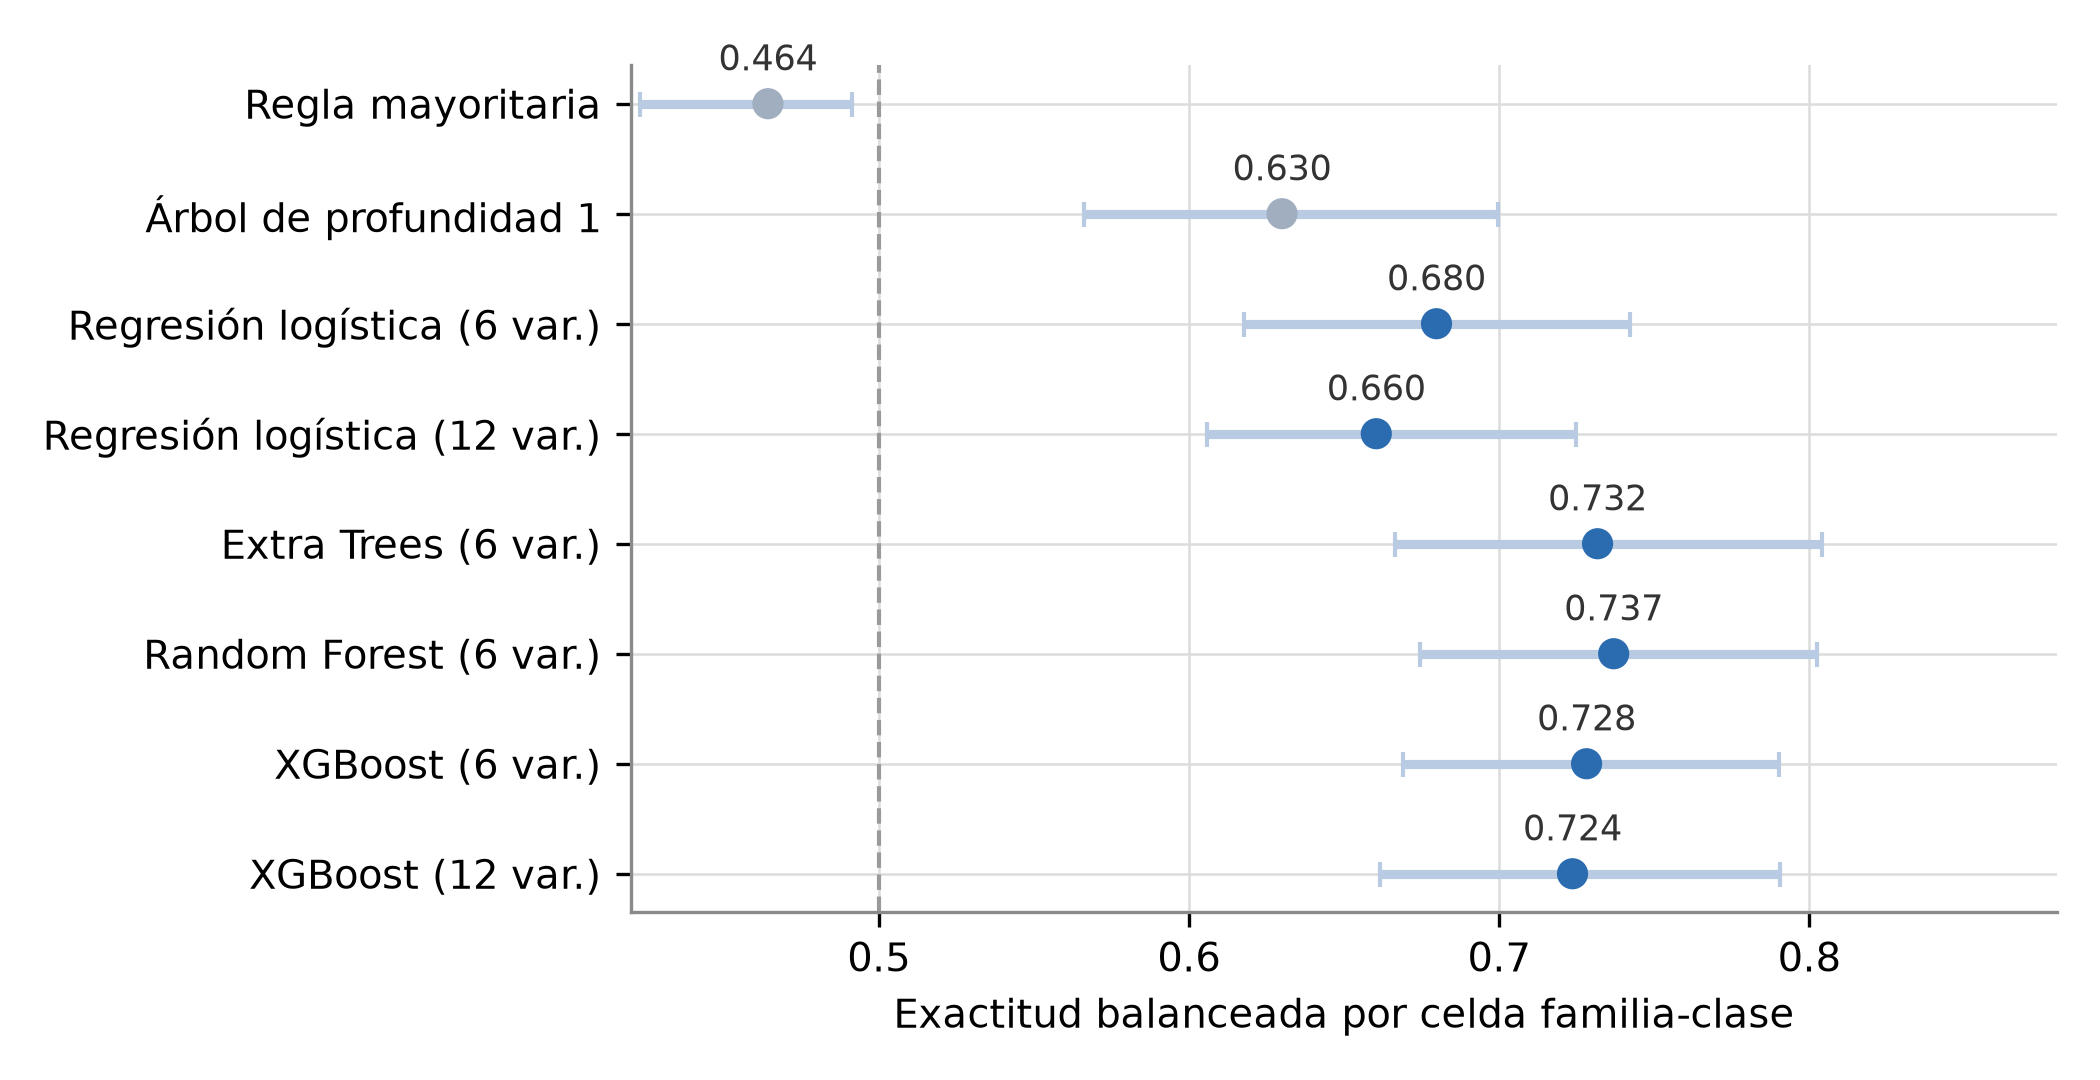
\includegraphics[width=\linewidth]{fig_cpu_comparacion_modelos_20260919.png}
    \end{column}
    \begin{column}{0.38\textwidth}
      \begin{cardhi}[halign=center]
        \bignum{0.728}\\
        XGBoost · exactitud balanceada por celda, familia retirada (IC95 0.669--0.790)
      \end{cardhi}
      \begin{card}
        Los bosques empatan dentro del IC95; XGBoost se eligió por latencia
        (243 µs frente a 5.3 ms en Python)
      \end{card}
      \begin{card}
        Optuna anidado: $+0.019$ (IC95 $-0.007$ a $+0.050$) → configuración fija.
        El límite está en la información, no en el modelo (anexo A5)
      \end{card}
    \end{column}
  \end{columns}
\end{frame}

% ---------------------------------------------------------------- OE2 GPU
\subseccion{Clasificador GPU}
\begin{frame}{En GPU se eligió el modelo que no depende del reloj que el agente modifica}
  \begin{columns}[c]
    \begin{column}{0.56\textwidth}
      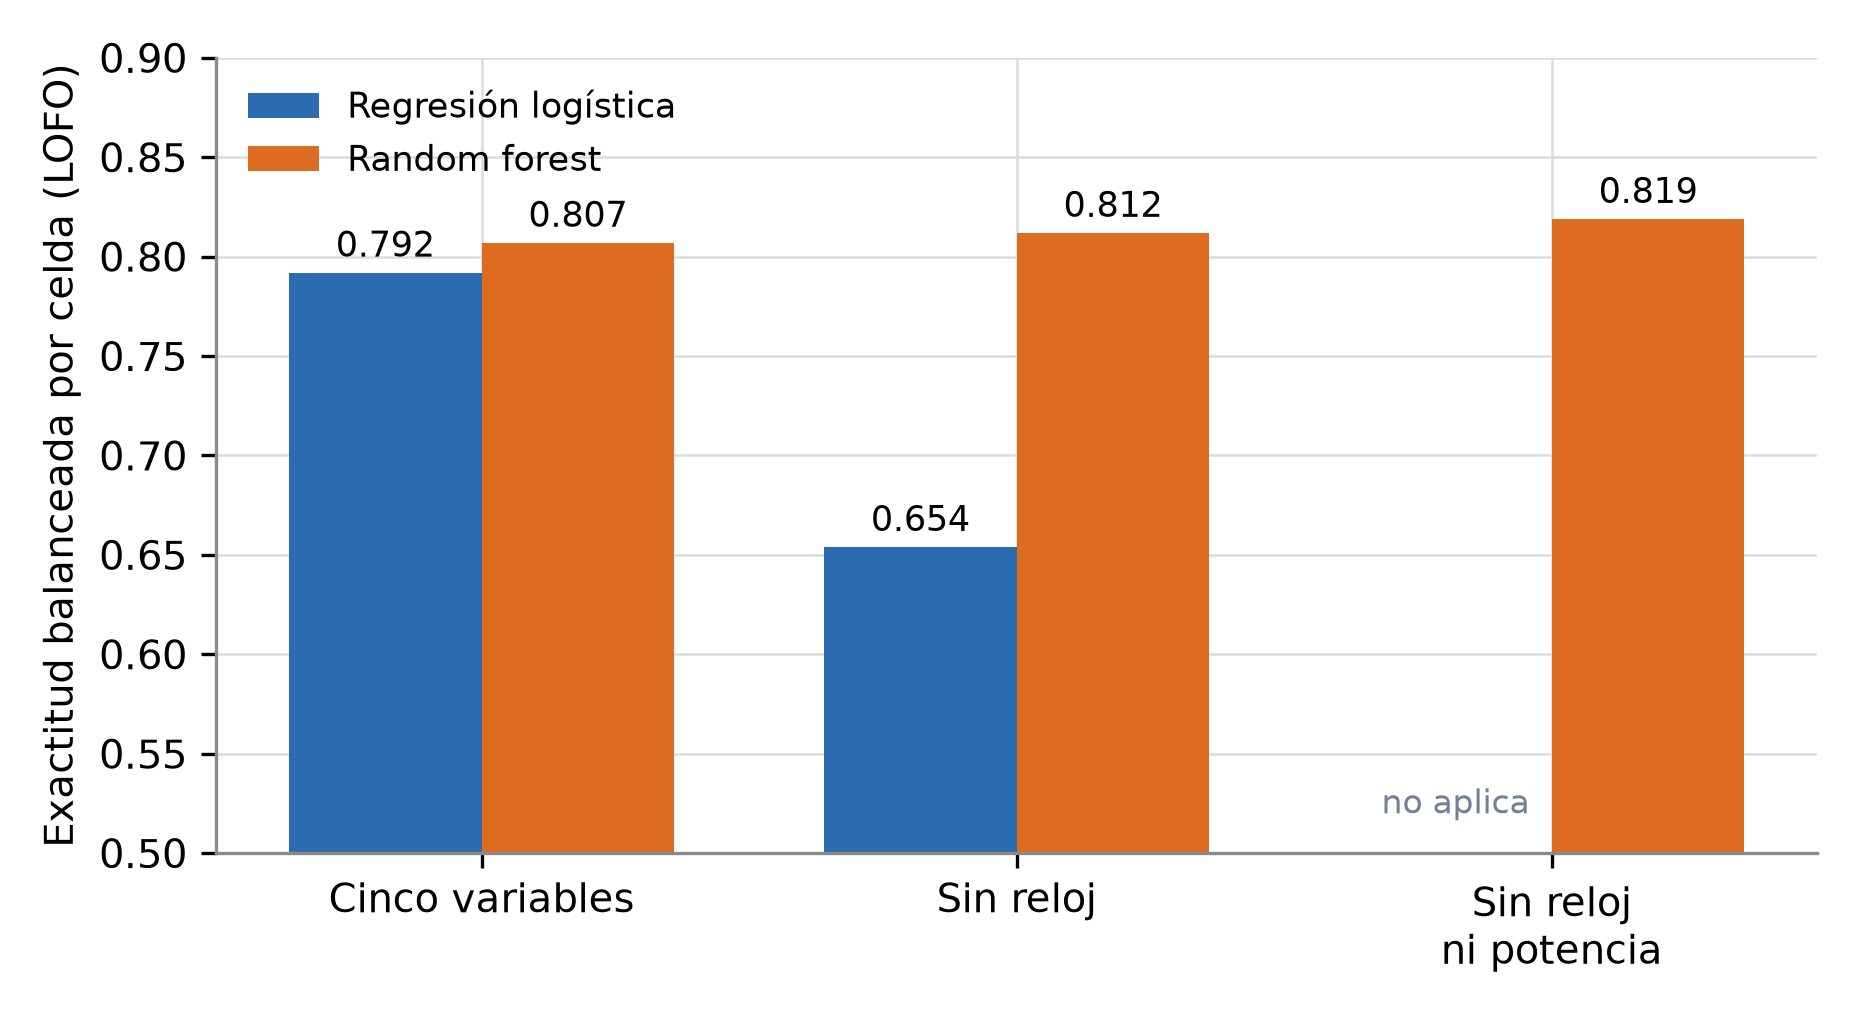
\includegraphics[width=\linewidth]{fig_gpu_invarianza_reloj_20260923.png}
    \end{column}
    \begin{column}{0.42\textwidth}
      \begin{cardhi}[halign=center]
        \bignum{0.819}\\
        \textit{Random forest} con 3 señales invariantes al reloj, familia retirada
      \end{cardhi}
      \begin{card}
        Fijar el reloj en 1410 MHz cambia el 26.7 \% de las predicciones de la
        regresión logística; el RF conserva su exactitud sin reloj ni potencia
      \end{card}
      \begin{card}
        Con $\tau=0.90$: 0.900 de exactitud y cobertura de 65.7 \%;
        0 errores en \textit{memory-bound}
      \end{card}
    \end{column}
  \end{columns}
\end{frame}

% ---------------------------------------------------------------- OE3
\subseccion{¿Es suficientemente rápida la inferencia?}
\begin{frame}{Inferir cuesta microsegundos; el proceso de CPU completo sí cuesta}
  \begin{columns}[c]
    \begin{column}{0.56\textwidth}
      \begin{tikzpicture}[x=0.8mm,y=1mm]
        % x = 10*(log10(t)+5) unidades  ->  10 us = 0, 10 s = 60
        \foreach \x/\l in {0/10 µs,20/1 ms,40/100 ms,60/10 s} {
          \draw[uisline!70] (\x,-1) -- (\x,-36);
          \node[font=\tiny,text=uisgray] at (\x,-39) {\l};}
        \lat{0}{2.0}{uisgreen}{Inferencia CPU}{16 µs}
        \lat{1}{9.9}{uisgreen}{Inferencia GPU}{97 µs}
        \lat{2}{24.5}{uismint}{Escritura de frecuencia CPU}{2.85 ms}
        \lat{3}{45.4}{uismint}{Cambio de reloj GPU}{0.35 s}
        \lat{4}{54.8}{uislime}{Ventana para decidir (GPU)}{3 s}
      \end{tikzpicture}

      {\tiny\color{uisgray} Escala logarítmica de tiempo.}
    \end{column}
    \begin{column}{0.42\textwidth}
      \begin{cardhi}
        \textbf{Proceso GPU (sombra):} EDP de 1.002 a 1.010 de la base; sin costo medible
      \end{cardhi}
      \begin{card}
        \textbf{Proceso CPU (sombra):} +5 a 9 \% de energía de CPU, unos 6 a 14 W,
        sin escribir ninguna frecuencia
      \end{card}
      \begin{card}
        \textbf{Matriz inicial:} CPU activo 1.15 y 1.06 de EDP; conjunto 1.04 y 1.06
        ($p=0.0079$)
      \end{card}
    \end{column}
  \end{columns}
  \vspace{1mm}
  {\scriptsize La sobrecarga de CPU no se atribuye a la inferencia: el proceso lee 9 contadores
  en 6 núcleos y decide unas mil veces por segundo.}
\end{frame}

% ---------------------------------------------------------------- política
\subseccion{¿La política produce un efecto medible?}
\begin{frame}{El piso de potencia decide la política: no actuar en CPU, F1 en GPU \textit{memory-bound}}
  \begin{columns}[c]
    \begin{column}{0.3\textwidth}
      \centering
      \begin{tikzpicture}[x=1mm,y=0.42mm]
        \fill[uisline!70] (0,0) rectangle (12,84);   \fill[uisgreen] (0,84) rectangle (12,100);
        \fill[uisline!70] (20,0) rectangle (32,55.8); \fill[uisgreen] (20,55.8) rectangle (32,100);
        \node[font=\tiny\bfseries] at (6,42) {84 \%};
        \node[font=\tiny\bfseries] at (26,28) {55.8 \%};
        \node[font=\tiny,text=white] at (6,92) {16 \%};
        \node[font=\tiny,text=white] at (26,78) {44 \%};
        \node[font=\scriptsize\bfseries] at (6,-8) {CPU};
        \node[font=\scriptsize\bfseries] at (26,-8) {GPU};
        \fill[uisline!70] (0,-22) rectangle ++(3,6); \node[font=\tiny,anchor=west] at (3.5,-19) {piso $P_0$};
        \fill[uisgreen] (17,-22) rectangle ++(3,6); \node[font=\tiny,anchor=west] at (20.5,-19) {dinámica};
      \end{tikzpicture}

      {\tiny\color{uisgray} Fracción de la potencia al reloj más alto.}
    \end{column}
    \begin{column}{0.68\textwidth}
      \scriptsize
      \renewcommand{\arraystretch}{1.35}
      \begin{tabularx}{\linewidth}{@{}l>{\raggedright\arraybackslash}X>{\raggedright\arraybackslash}X@{}}
        \toprule
        & \textbf{compute-bound} & \textbf{memory-bound}\\
        \midrule
        \textbf{CPU} & No actuar\newline{\tiny\color{uisgray}F0 mejora 0.56 \%, bajo el mínimo de 1 \%}
                     & No actuar\newline{\tiny\color{uisgray}F1 empeora 5.4 \% (IC95 3.4 a 6.8)}\\
        \textbf{GPU} & No actuar\newline{\tiny\color{uisgray}F1 +2.1 \% (IC95 $-12.7$ a 14.2; $p=0.438$)}
                     & \textbf{F1 = 1260 MHz}\newline{\tiny\color{uisgray}+8.9 \% de EDP GPU (IC95 3.0 a 13.3), estimación interna;
                       \textbf{6.5 \%} con la familia fuera (IC95 $-4.0$ a 13.1)}\\
        \bottomrule
      \end{tabularx}
      \vspace{2mm}

      En CPU, bajar a 0.8 GHz ahorra solo 15 \% de potencia; ni un oráculo por kernel
      pasa de 2.2 \% de mejora media. Excepción en GPU: \texttt{rodinia\_gaussian}
      es \textit{memory-bound} pero pierde 27.3 \% con F1.
    \end{column}
  \end{columns}
\end{frame}

% ---------------------------------------------------------------- OE4
\subseccion{¿Cómo se compara con la base nativa?}
\begin{frame}{Con fases de memoria largas, el agente de GPU reduce el EDP CPU+GPU 3.8--3.9 \%}
  \begin{columns}[c]
    \begin{column}{0.58\textwidth}
      \begin{tikzpicture}[x=6mm,y=1mm]
        % eje x en %: -8 .. +1 ; 1 % = 6 mm
        \foreach \v in {-8,-6,-4,-2,0} {
          \draw[uisline!70] (\v,-1) -- (\v,-43);
          \node[font=\tiny,text=uisgray] at (\v,-46) {\v\,\%};}
        \draw[uisgray,line width=0.6pt] (0,-1) -- (0,-43);
        \node[font=\scriptsize\bfseries,anchor=west] at (0.3,-6) {EDP CPU+GPU};
        \gbar{-6}{-3.8}{-5.4}{-2.3}{uisgreen}{$-3.8$ \%}
        \gbar{-11}{-3.9}{-4.6}{-3.2}{uislime}{$-3.9$ \%}
        \node[font=\scriptsize\bfseries,anchor=west] at (0.3,-21) {Energía GPU};
        \gbar{-21}{-7.2}{-7.7}{-6.8}{uisgreen}{$-7.2$ \%}
        \gbar{-26}{-6.4}{-7.6}{-5.3}{uislime}{$-6.4$ \%}
        \node[font=\scriptsize\bfseries,anchor=west] at (0.3,-36) {Duración};
        \gbar{-36}{-0.8}{-1.6}{0.1}{uisgreen}{$-0.8$ \%}
        \gbar{-41}{0.1}{0.0}{0.2}{uislime}{$+0.1$ \%}
        \fill[uisgreen] (-8,7) rectangle ++(0.4,2.5); \node[font=\tiny,anchor=west] at (-7.5,8.2) {E-A};
        \fill[uislime] (-6,7) rectangle ++(0.4,2.5); \node[font=\tiny,anchor=west] at (-5.5,8.2) {CloverLeaf};
        \node[font=\tiny,text=uisgray,anchor=west] at (-8,2.5) {media geométrica por bloque · bigotes: IC95};
      \end{tikzpicture}
    \end{column}
    \begin{column}{0.4\textwidth}
      \begin{cardhi}
        \textbf{5 de 5 bloques} favorables en ambas ($p=0.0625$, el mínimo posible con 5):
        dirección consistente, IC95 calculado \textit{post hoc}
      \end{cardhi}
      \begin{card}
        \textbf{Brazo sombra ≈ paridad} (0.997): el ahorro viene de actuar, no de observar
      \end{card}
      \begin{card}
        \textbf{Con \textit{powersave}:} $-2.6$ \% y $-3.2$ \%; mismas conclusiones
      \end{card}
      \begin{card}
        \textbf{Pero:} en E-A, un reloj fijo en F1 logra lo mismo (agente/F1 fijo = 0.998)
      \end{card}
    \end{column}
  \end{columns}
  \notapie{E-A: compuesta con familias vistas, fases de memoria de 46 a 60 s. CloverLeaf CUDA Fortran: aplicación externa. En E-A la CPU es \textasciitilde 64 \% de la energía medida y no se modifica.}
\end{frame}

\subseccion{¿Aporta clasificar por fase?}
\begin{frame}{Clasificar supera al reloj fijo cuando una fase de cómputo depende del reloj}
  \centering
  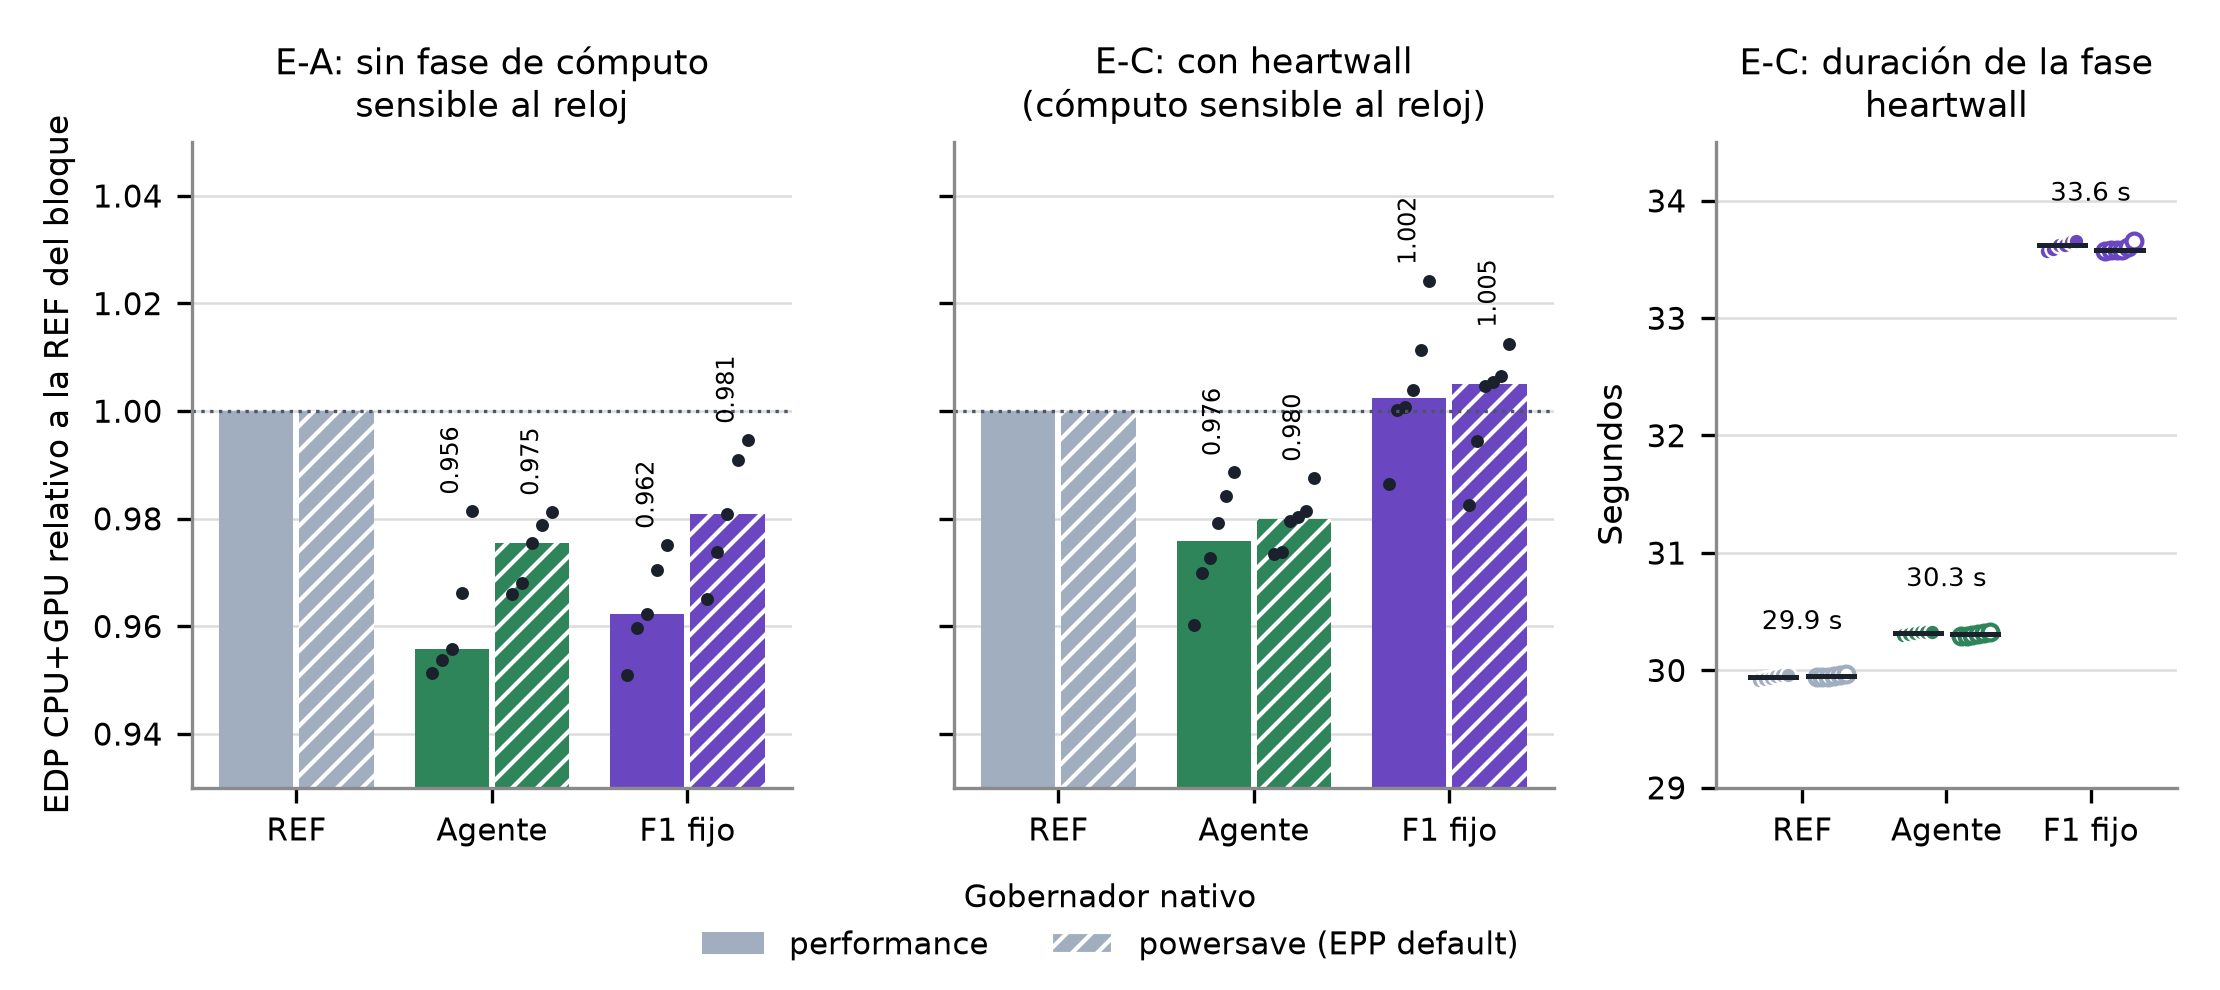
\includegraphics[width=0.66\textwidth]{fig_fase4_EC_20260930.png}

  \vspace{1mm}
  \begin{minipage}[t]{0.32\textwidth}
    \begin{card}[height=13mm,valign=center,fontupper=\tiny]
      \textbf{E-A:} agente/F1 fijo = 0.998 (IC95 0.990--1.006). DGEMM ya corría bajo 1260 MHz
      por el límite de potencia
    \end{card}
  \end{minipage}\hfill
  \begin{minipage}[t]{0.32\textwidth}
    \begin{cardhi}[height=13mm,valign=center,fontupper=\tiny]
      \textbf{E-C:} agente/F1 fijo = \textbf{0.972} (IC95 0.958--0.985); 6 de 6 bloques,
      $p=0.031$. Frente a la base: 0.976 ($p=0.031$)
    \end{cardhi}
  \end{minipage}\hfill
  \begin{minipage}[t]{0.32\textwidth}
    \begin{card}[height=13mm,valign=center,fontupper=\tiny]
      \textbf{heartwall:} 29.9 s base · 30.3 s agente · 33.6 s F1 fijo.
      F1 fijo no mejora la base (1.004)
    \end{card}
  \end{minipage}
  \notapie{E-C es una prueba de mecanismo: escenario construido con el kernel más favorable y una familia vista. En E-B (exploratorio), cuando el agente se abstuvo, F1 fijo ahorró más.}
\end{frame}

\subseccion{¿Qué no funcionó?}
\newcommand{\nocard}[2]{%
  \begin{card}[height=19mm,valign=center]
    \begin{tabular}{@{}m{8mm}@{}m{0.8\linewidth}@{}}
      \nomark & {\footnotesize\bfseries #1}\par\vspace{0.6mm}{\scriptsize #2}
    \end{tabular}
  \end{card}}
\begin{frame}{El agente no ganó en CPU, en LAMMPS ni en familias GPU no vistas}
  \vspace{4mm}
  \begin{columns}[T]
    \begin{column}{0.48\textwidth}
      \nocard{CPU}{Piso de potencia del 84 \%: la política es no actuar y el proceso de observación aumenta el EDP}
      \nocard{Familias GPU inéditas}{BabelStream: abstención en 9 de 11 repeticiones (E-B); quedó cerca de la paridad}
    \end{column}
    \begin{column}{0.48\textwidth}
      \nocard{LAMMPS}{EDP entre 1.003 y 1.009 de la base; el agente nunca aplicó F1}
      \nocard{Alcance}{Un solo nodo; modelo GPU entrenado por corrida y aplicado en ventanas de 3~s}
    \end{column}
  \end{columns}
\end{frame}

% ---------------------------------------------------------------------
%  08 · Conclusiones
% ---------------------------------------------------------------------
\seccion{Conclusiones}

% hallazgo: número, cifra, título, explicación
\newcommand{\hallazgo}[4]{%
  \begin{card}[height=17mm,valign=center]
    \begin{tabular}{@{}>{\centering\arraybackslash}m{9mm}@{\hspace{2mm}}>{\centering\arraybackslash}m{32mm}@{\hspace{3mm}}>{\raggedright\arraybackslash}m{0.56\linewidth}@{}}
      \badge{#1} & {\large\bfseries\boldmath\color{uisgreen}#2} &
      {\small\bfseries #3}\par\vspace{0.5mm}{\footnotesize\color{uisgray}#4}
    \end{tabular}
  \end{card}}

\begin{frame}{Tres hallazgos}
  \vspace{1mm}
  \hallazgo{1}{84 \% vs 55.8 \%}{El piso de potencia decide dónde vale la pena el DVFS}
    {En CPU casi toda la potencia es piso y no hay margen; en GPU sí}
  \hallazgo{2}{0.819}{Señales ligeras aproximan el régimen Roofline sin perfilar}
    {En familias no vistas, con inferencia de 97 µs; perfilar con Nsight alarga 60 veces la ejecución}
  \hallazgo{3}{$-2.8$ \%}{Clasificar por fase gana cuando hay cómputo sensible al reloj}
    {Frente a un reloj fijo en E-C; donde no hay esa fase (E-A), una regla fija rinde igual}
\end{frame}

% fila de respuesta: parte de la pregunta, GPU, CPU
\newcommand{\resp}[5][13]{%
  \fill[uiscard,rounded corners=1mm] (0,#2) rectangle (126,{#2+#1});
  \node[font=\small\bfseries,anchor=west,align=flush left,text width=39mm] at (3,{#2+#1/2}) {#3};
  \node[font=\small,anchor=west,align=flush left,text width=38mm] at (47,{#2+#1/2}) {#4};
  \node[font=\small,anchor=west,align=flush left,text width=36mm] at (88,{#2+#1/2}) {#5};}

\begin{frame}{Respuesta a la pregunta de investigación}
  \centering
  \begin{tikzpicture}[x=1mm,y=1mm]
    \node[font=\small\bfseries,text=uisgreen,anchor=west] at (49,53.5) {GPU};
    \node[font=\small\bfseries,text=uisred,anchor=west] at (90,53) {CPU};
    \resp[18]{32}{¿Reduce el\\consumo?}
      {\textbf{Sí:} $-3.8$ / $-3.9$ \% de EDP CPU+GPU\\[0.3mm]{\footnotesize\color{uisgray}solo GPU: $-8.0$ / $-6.3$ \%; con memoria larga}}
      {\textbf{No:} con un piso de 84 \% no hay margen}
    \resp{17}{¿La inferencia\\degrada el rendimiento?}
      {\textbf{No:} 97 µs por decisión; la duración no cambia}
      {\textbf{No es inferir} (16 µs): observar sube 5--9 \% la energía de CPU}
    \resp{2}{¿Frente a los\\gobernadores nativos?}
      {\textbf{Se mantiene} con \textit{performance} y \textit{powersave}}
      {Empeora el EDP con ambos}
    \fill[uisgreen,rounded corners=1mm] (0,-12) rectangle (126,-2);
    \node[font=\normalsize\bfseries,text=white] at (63,-7) {Recomendación: desplegar solo el proceso de GPU};
  \end{tikzpicture}
\end{frame}

% tarjeta de límite: título, texto
\newcommand{\limite}[2]{%
  \begin{card}[height=21mm,valign=top]
    {\small\bfseries\color{uisgreen}#1}\par\vspace{0.8mm}{\footnotesize #2}
  \end{card}}

\begin{frame}{Limitaciones: qué no afirma este trabajo}
  \vspace{1mm}
  \begin{columns}[T]
    \begin{column}{0.32\textwidth}
      \limite{Un solo nodo}{Xeon Gold 5315Y + A100. No se generaliza a otras CPU, GPU ni controladores}
      \limite{CPU acotada}{Solo la frecuencia de 6 núcleos delegados, sin turbo ni \textit{uncore}. No es la CPU completa}
    \end{column}
    \begin{column}{0.32\textwidth}
      \limite{Energía medida}{Paquetes de CPU y GPU. No incluye DRAM, placa, fuente ni ventilación: no es la energía del nodo}
      \limite{Gobernadores}{\textit{performance} y \textit{powersave}; \textit{ondemand} y \textit{schedutil} no existen con \texttt{intel\_pstate}}
    \end{column}
    \begin{column}{0.32\textwidth}
      \limite{Evidencia}{5 bloques: dirección consistente, no confirmación. E-C es una prueba de mecanismo construida}
      \limite{Modelo de GPU}{Entrenado por corrida y aplicado en ventanas de 3 s; con fases cortas o familias nuevas se abstiene}
    \end{column}
  \end{columns}
\end{frame}

% elemento de lista con viñeta verde
\newcommand{\vineta}[1]{\par\vspace{1.6mm}\noindent\textcolor{uisgreen}{\rule[0.5ex]{1.6mm}{1.6mm}}\hspace{2mm}#1}

\begin{frame}{Trabajo futuro}
  \vspace{4mm}
  \begin{cardhi}[width=0.86\textwidth,center]
    \small
    \vineta{Más familias externas \textit{memory-bound} en GPU, evaluadas una sola vez con el modelo congelado}
    \vineta{Repetir base, agente y F1 fijo en aplicaciones externas con cómputo sensible al reloj}
    \vineta{Reentrenar el modelo de GPU por ventana, con fronteras de fase de CUPTI}
    \vineta{Reducir primero el costo de observar en CPU, antes de revisar su política}
    \vineta{Probar en otras arquitecturas con un piso de potencia de CPU más bajo, donde el DVFS de CPU sí tenga margen}
    \vineta{Actuar también sobre la frecuencia del \textit{uncore} y de la memoria en CPU, no solo sobre la de los núcleos}
  \end{cardhi}
\end{frame}

% ---------------------------------------------------------------------
%  Cierre
% ---------------------------------------------------------------------
\begin{frame}[plain]
  \centering
  \vspace{6mm}
  {\fontsize{30}{32}\selectfont\bfseries\color{uisgreen} Gracias\par}
  \vspace{5mm}
  {\footnotesize Yeison Adrián Cáceres Torres · Ricardo Andrés Pérez Porras\\
   Director: Gilberto Javier Díaz Toro, Ph.D.\par}
  \vspace{3mm}
  {\scriptsize\color{uisgray} Repositorio: \texttt{github.com/AdrianCCRS/hyperion}\par}
  \vspace{6mm}
  
\includegraphics[height=9mm]{logos/cage.png}\hspace{4mm}%
  
\includegraphics[height=9mm]{logos/uis.png}
\end{frame}


\appendix
\AtBeginSection[]{}
% ---------------------------------------------------------------------
%  Anexo
%  \figanexo{código}{rótulo}{título}{figura}{ancho}{tarjeta 1}{tarjeta 2}{tarjeta 3}
%  La tercera tarjeta se dibuja destacada. (El rótulo #2 queda solo como referencia.)
% ---------------------------------------------------------------------
\section{Anexo}

\newcommand{\figanexo}[8]{%
  \begin{frame}{#1 · #3}
    \begin{columns}[c]
      \begin{column}{0.68\textwidth}
        \centering\includegraphics[width=#5\linewidth,height=0.72\textheight,keepaspectratio]{#4}
      \end{column}
      \begin{column}{0.3\textwidth}
        \begin{card}#6\end{card}
        \begin{card}#7\end{card}
        \begin{cardhi}#8\end{cardhi}
      \end{column}
    \end{columns}
  \end{frame}}

\begin{frame}{Índice del anexo}
  \vspace{2mm}
  \footnotesize
  \begin{columns}[T]
    \begin{column}{0.48\textwidth}
      \begin{card}
        \textbf{Fase 1 · Medición}\par
        A1 Composición de clase por familia\par
        A2 Validación de la medición
      \end{card}
      \begin{card}
        \textbf{Fase 2 · Clasificador CPU}\par
        A3 Matrices de confusión\par
        A4 Resultado por familia\par
        A5 Perfiles gemelos\par
        A6 Abstención
      \end{card}
      \begin{card}
        \textbf{Fase 2 · Clasificador GPU}\par
        A7 Matrices de confusión\par
        A8 Invarianza al reloj
      \end{card}
    \end{column}
    \begin{column}{0.48\textwidth}
      \begin{card}
        \textbf{Fase 3 · Política y agente}\par
        A9 Política CPU\par
        A10 Energía relativa CPU\par
        A11 Política GPU\par
        A12 Energía relativa GPU\par
        A13 Verificación del agente
      \end{card}
      \begin{card}
        \textbf{Fase 4 · Evaluación}\par
        A14 Aplicaciones compuestas\par
        A15 Matriz inicial\par
        A16 Potencial de la GPU\par
        A17 Escenario E\par
        A18 CloverLeaf\par
        A19 LAMMPS
      \end{card}
    \end{column}
  \end{columns}
\end{frame}

% ----------------------------------------------------------------- Fase 1 · Medición
\figanexo{A1}{CPU · Fase 1}{Composición de fase por familia en CPU}
  {fig_cpu_composicion_clase_por_familia_20260925.png}{1}
  {1\,309\,755 intervalos elegibles (91.9 \%): 40.2 \% \textit{compute}, 59.8 \% \textit{memory}}
  {La fracción \textit{compute} sube de 29.0 \% (nativo) a 46.4 \% (F8) porque el \textit{ridge} baja}
  {Familias mixtas (npb\_bt, npb\_lu, cholmod, phasic…) aportan ejemplos cerca del \textit{ridge}}

\begin{frame}{A2 · Validación de la medición: techos y frecuencia efectiva}
  \vspace{3mm}
  \begin{columns}[T]
    \begin{column}{0.48\textwidth}
      \begin{card}[height=19mm]
        {\footnotesize\bfseries Ancho de banda}\par
        Calibrado 58.4--58.8 GB/s frente a 64.0--66.8 GB/s de Intel Advisor (8--13 \% por debajo)
      \end{card}
      \begin{card}[height=19mm]
        {\footnotesize\bfseries \textit{Ridge} nativo}\par
        Advisor lo ubica entre 7.1 y 9.5 FLOP/B; la campaña usó 8.69 FLOP/B
      \end{card}
    \end{column}
    \begin{column}{0.48\textwidth}
      \begin{card}[height=19mm]
        {\footnotesize\bfseries Techo de cómputo}\par
        417.8--555 GFLOP/s, consistente con 577.7 GFLOP/s de Advisor en los mismos seis núcleos
      \end{card}
      \begin{cardhi}[height=19mm]
        {\footnotesize\bfseries Frecuencia efectiva}\par
        Restringir también los hermanos SMT llevó la razón de rendimiento F0/F8 de 0.995 a 3.78 (esperado ≈ 4)
      \end{cardhi}
    \end{column}
  \end{columns}
\end{frame}


% ----------------------------------------------------------------- Fase 2 · Clasificador CPU
\figanexo{A3}{CPU · Fase 2}{Matrices de confusión y métricas del clasificador CPU}
  {fig_cpu_matriz_confusion_20260919.png}{1}
  {Exactitud 0.769 · F1 macro 0.760 · AUC 0.842 · MCC 0.520}
  {Sensibilidad: \textit{compute} 0.714, \textit{memory} 0.806}
  {Con $\tau=0.85$ (derecha), F1 macro 0.842, pero refleja sobre todo qué intervalos quedan fuera}

\figanexo{A4}{CPU · Fase 2}{El resultado en CPU varía mucho entre familias}
  {fig_cpu_resultado_por_familia_20260919.png}{0.8}
  {\textbf{14} familias superan 0.9 de exactitud}
  {\textbf{5} quedan por debajo de 0.55; npb\_ft en \textbf{0.314}}
  {Las peores tienen un perfil de contadores igual al de familias de la clase contraria}

\figanexo{A5}{CPU · Fase 2}{El límite está en la información: perfiles gemelos}
  {fig_cpu_perfiles_gemelos_20260922.png}{1}
  {gap\_pr (\textit{memory}) y la fase \textit{compute} de phasic: MPKI 0.82 vs 0.94, IPC 1.11 vs 0.97}
  {kNN sin ajuste: 0.684; curva de aprendizaje 0.615 → 0.718 (3 a 23 familias)}
  {Con $I$ como entrada se llega a 0.9989: la brecha es información que las seis señales no transportan}

\figanexo{A6}{CPU · Fase 2}{Abstención en CPU: $\tau=0.85$ decide el 72.2 \%}
  {fig_cpu_umbral_calibracion_20260919.png}{1}
  {Sobre lo decidido sube solo de 0.728 a 0.738; abstenerse al azar no mejora}
  {Sobreconfianza fuera de familia: confianza media 0.890, exactitud 0.764 (ECE 0.126)}
  {Con confianza $\ge 0.9$, npb\_ft acierta 32 \% y npb\_mg 35 \%}


% ----------------------------------------------------------------- Fase 2 · Clasificador GPU
\figanexo{A7}{GPU · Fase 2}{Matrices de confusión del \textit{random forest} de GPU}
  {fig_gpu_rf_matriz_confusion.png}{1}
  {Exactitud 0.892 · F1 macro 0.881 · AUC 0.913 · MCC 0.763}
  {Con $\tau=0.90$: 0.900, cobertura por celda 65.7 \%; 0 errores en \textit{memory}}
  {De 239 corridas que activarían F1, 224 son \textit{memory} (precisión 0.937)}

\figanexo{A8}{GPU · Fase 2}{Por qué el modelo de GPU no usa el reloj ni la potencia}
  {fig_gpu_invarianza_reloj_20260923.png}{1}
  {Al fijar el reloj en 1410 MHz, la regresión logística cambia de clase el 26.7 \% de sus predicciones}
  {Sin el reloj, la regresión logística baja a 0.654; el \textit{random forest} no pierde nada}
  {Frente a \textit{extra trees}: mayor sensibilidad (0.809 y 0.891 vs 0.749 y 0.855), menor variación entre semillas y \textit{dual\_cholesky} 0.51 vs 0.15}


% ----------------------------------------------------------------- Fase 3 · Política y agente
\figanexo{A9}{Fase 3}{Política CPU: no actuar en ninguna clase}
  {fig_cpu_politica_forest_20260922.png}{1}
  {Cómputo: F0 mejora 0.56 \%, menos que el efecto mínimo de 1 \%}
  {Memoria: F1 empeora 5.4 \% (IC95 3.4 a 6.8)}
  {Un oráculo por kernel ganaría 2.2 \% en promedio; 22 de 47 kernels bajo 1 \%}

\figanexo{A10}{Fase 3}{En CPU el tiempo crece más de lo que cae la potencia}
  {fig_cpu_energia_relativa_20260920.png}{1}
  {La energía de memoria se mantiene cerca de la referencia hasta \textasciitilde 2 GHz}
  {Con $P(f)=P_0+c\,f^k$, bajar el reloj mejora el EDP solo si $\beta<\beta_{\text{crít}}$}
  {$\beta_{\text{crít}}$: mediana 0.14, máximo 0.33; el cómputo denso tiene $\beta\approx1$}

\figanexo{A11}{Fase 3}{Política GPU: no actuar en cómputo, F1 en memoria}
  {fig_gpu_politica_forest_20260922.png}{1}
  {Cómputo: F1 +2.1 \% (IC95 $-12.7$ a 14.2; $p=0.438$) → no actuar}
  {Memoria: F1 +8.9 \% (IC95 3.0 a 13.3; $p=0.020$), estimación interna; con la familia fuera, 6.5 \% (IC95 $-4.0$ a 13.1)}
  {rodinia\_gaussian pierde 27.3 \%: $\beta=0.941$ pese a ser \textit{memory-bound}}

\figanexo{A12}{Fase 3}{En GPU la energía de memoria cae hasta F3}
  {fig_gpu_politica_energia_relativa_20260922.png}{1}
  {Piso estático $P_0=38.5$ W: 55.8 \% de la potencia al reloj más alto (CPU: 84 \%)}
  {$\beta$ mediano: \textit{compute} 0.837, \textit{memory} 0.189}
  {EDP $<1$ en F1--F2 para \textit{memory}; desde F5 domina el tiempo}

\newcommand{\vcard}[2]{\begin{card}[height=21mm,valign=top]{\footnotesize\bfseries #1}\par\vspace{0.6mm}#2\end{card}}

\begin{frame}{A13 · Verificación del agente antes de la evaluación}
  \vspace{2mm}
  \begin{columns}[T]
    \begin{column}{0.32\textwidth}
      \vcard{Exportación ONNX}{Diferencia máx.\ de probabilidad $3\times10^{-7}$ (CPU) y $9\times10^{-8}$ (GPU); ninguna etiqueta cambia}
      \vcard{Coordinación}{Con ambos procesos activos, el piso de CPU de 3.2 GHz se respetó en el 99.2 \% de las muestras}
    \end{column}
    \begin{column}{0.32\textwidth}
      \vcard{Latencias}{Inferencia 16.4 µs (CPU) y 97 µs (GPU); escritura CPU 2.85 ms en paralelo; cambio de reloj GPU 0.35--0.37 s}
      \vcard{Premisa física}{Con el reloj fijado, \textit{compute} escala con el reloj y \textit{memory} no cae hasta 510 MHz}
    \end{column}
    \begin{column}{0.32\textwidth}
      \vcard{Restauración}{Ante SIGTERM o SIGINT devolvió reloj GPU, turbo y rango de CPU al estado inicial, código de salida 0}
      \vcard{Permanencia mínima GPU}{3.7 s: diez veces la latencia de un cambio completo}
    \end{column}
  \end{columns}
\end{frame}


% ----------------------------------------------------------------- Fase 4 · Evaluación
\figanexo{A14}{Fase 4}{Aplicaciones compuestas y clasificación en el lazo}
  {fig_fase4_aplicaciones_20260926.png}{1}
  {Tiempo en fases \textit{memory}: de 15 \% (B, CPU) a 71 \% (A)}
  {CPU: acierta 96.7--97.5 \% (vistas) y 99.6--99.8 \% (inéditas), ponderado por ventanas}
  {GPU: ninguna decisión errónea; se abstuvo en 2/12 (A) y 4--5/12 (B)}

\figanexo{A15}{Fase 4}{Matriz inicial: el proceso de CPU empeora el EDP}
  {fig_fase4_edp_alcance_20260930.png}{1}
  {GPU activo: EDP 1.00 en A y B; sombra 1.01 y 1.00}
  {CPU activo: 1.15 (A) y 1.06 (B); conjunto 1.04 y 1.06 ($p=0.0079$)}
  {Sombra CPU ya en 1.10 y 1.05: +13.6 W y +6.2 W a igual duración}

\figanexo{A16}{Fase 4}{Potencial de la GPU en la matriz inicial}
  {fig_fase4_gpu_potencial_20260930.png}{1}
  {Esperado (fracción \textit{memory} × 8.9 \%): 3.2 \% (A) y 4.3 \% (B) de EDP GPU}
  {Medido: 0.5 \% y 3.0 \% de EDP GPU; 0.1 y 0.2 \% del EDP CPU+GPU; no se separa de cero}
  {En B, 4 de 6 decisiones sobre BabelStream fueron abstenciones: motivó el escenario E}

\figanexo{A17}{Fase 4}{Escenario E: fases de memoria largas}
  {fig_fase4_E_20260930.png}{0.85}
  {E-A: agente 0.962 de EDP CPU+GPU (IC95 0.946--0.977); energía GPU 0.928}
  {F1 fijo 0.964; agente/F1 fijo = 0.998 (IC95 0.990--1.006)}
  {E-B: sombra 1.028 y activo 1.016 (descriptivo); myocyte bimodal}

\figanexo{A18}{Fase 4}{CloverLeaf: una decisión sostenida en una aplicación externa}
  {fig_fase4_cloverleaf_20260930.png}{1}
  {Una decisión \textit{memory-bound} con confianza 1.00 a los \textasciitilde 3 s; resultado físico idéntico ($10^{-8}$)}
  {EDP CPU+GPU 0.961 (IC95 0.954--0.968); energía GPU 0.936; duración 1.001}
  {Se comporta como F1 fijo mientras la GPU está activa; F1 fijo no se midió aquí}

\figanexo{A19}{Fase 4}{LAMMPS: paridad con la base}
  {fig_fase4_D_20260930.png}{1}
  {GPU activo entre 1.003 y 1.009 de la base según la entrada}
  {chain y rhodo: sin decisiones; lj y eam: solo \textit{compute} → nunca F1}
  {Con el agente de CPU en observación: +2.9 a 3.4 \% de EDP}



\end{document}
